\documentclass[a4paper]{article}
\usepackage[a4paper,pdftex]{geometry}
\usepackage[english]{babel}
\usepackage{amsmath,amsfonts}
\usepackage[pdftex]{graphicx}
\usepackage{epstopdf}
\usepackage{fancyhdr}
\usepackage{lastpage}
\usepackage{setspace}
\usepackage{xcolor}
\usepackage{hyperref}
\usepackage{url}
\usepackage[all]{xy}
\usepackage[toc,page]{appendix}
\usepackage[T1]{fontenc}   

% Page style
\pagestyle{fancy}

% Page numbering
\lhead{}
\cfoot{}
\rfoot{\thepage}

\author{Chiel Kooijman\\5743028\\\url{Chiel999@gmail.com} \and
Steven Laan\\6036031\\\url{S.Laan@uva.nl} \and
Camiel Verschoor\\10017321\\\url{Verschoor@uva.nl} \and
Auke Wiggers\\6036163\\\url{A.J.Wiggers@uva.nl}}

\title{Collaborative Visual SLAM\\\normalsize Multi-Agent Visual Odometry and SLAM with humanoid robots.\\Project AI (6 EC)\\Artificial Intelligence\\Faculty of Science\\University of Amsterdam}

\begin{document}

%% FRONT PAGE
\thispagestyle{empty}
\begin{center}
\Large\textsc{Collaborative Visual SLAM}\\
\normalsize\textsc{Multi-Agent Visual Odometry and SLAM with humanoid robots.}

\vspace{2cm}

\begin{figure*}[!ht]
\centering
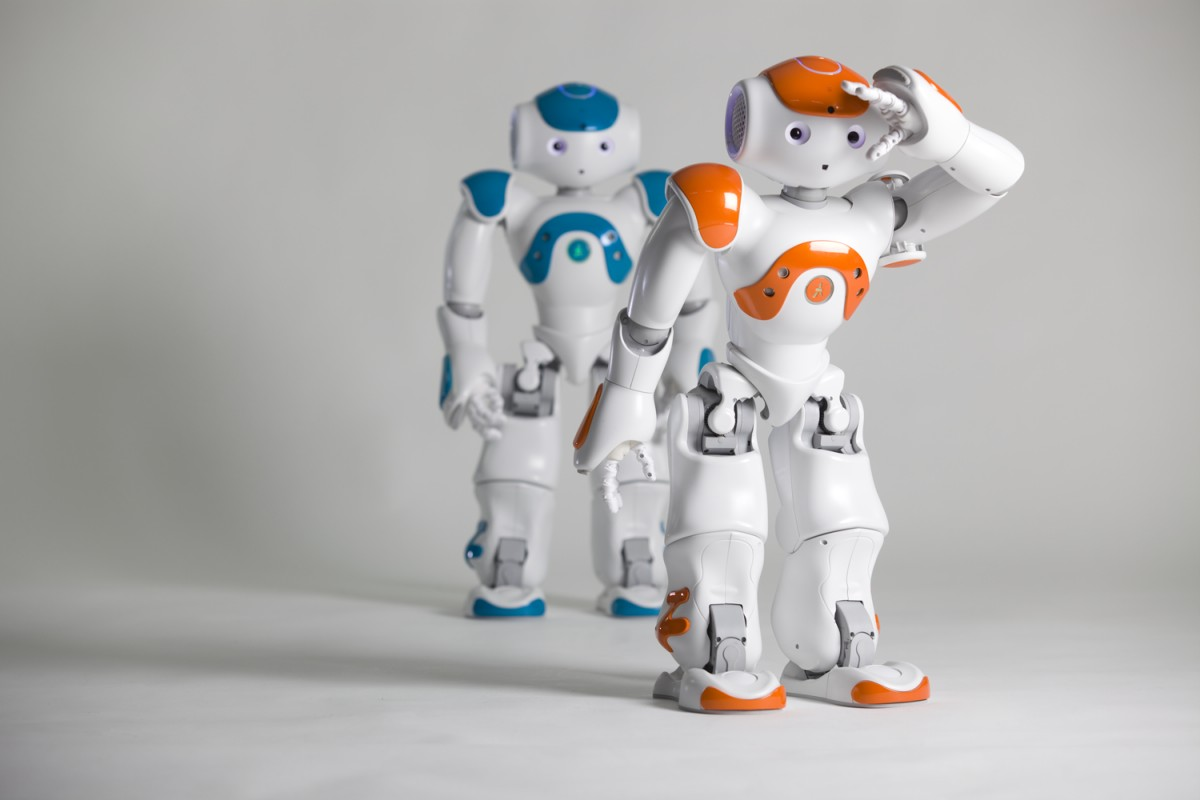
\includegraphics[width=\textwidth]{images/front.jpg}
\end{figure*}

\subsubsection*{An Artificial Intelligence project by Auke J. Wiggers, Camiel R. Verschoor,\\Chiel Kooijman and Steven Laan}
\end{center}

\newpage

% EMPTY PAGE
\thispagestyle{empty}
\mbox{}
\newpage

% OFFICIAL FRONT PAGE
\maketitle
\clearpage

% TABLE OF CONTENTS
\thispagestyle{empty}
\tableofcontents
\clearpage

\section{Introduction}

\section{Related Work}

\section{Theory}

\section{Pipeline}
In this section, the pipeline of our proposed system is described stepwise.

\begin{figure}[!hb]
\centerline{
\xymatrix{
Calibration\ar[d]\\
Egomotion\ar[d]\\
Reconstruction\ar[d]\\
Modelling\ar[d]\\
Combining Visual Odometry
}
}
\caption{Schematic overview of the pipeline of the system}
\label{fig:system}
\end{figure}

\subsection{Calibration}
Camera calibration is the process of estimating the intrinsic (and mostly the extrensic) parameters of the camera. Barrel distortion occurs in images taken the Nao robot's camera. Camera calibration allows the removal of this camera distortion.
\par
Description of method used for calibration.


\subsection{Egomotion}
Egomotion is the process of estimating a camera's motion relative to a rigid scene. There are two main approaches for estimating the relative motion between two frames, namely, Image-to-Image and Image-to-World.


\subsubsection{Feature extraction}
In this section, we concisely describe the feature extraction methods that were used in the system to extract features. In total three feature extractions methods were applied, namely, Binary Robust Invariant Scalable Keypoints (BRISK) \cite{Leutenegger2011}, Oriented FAST and Rotated BRIEF (ORB) \cite{Rublee2011} and Fast Retina Keypoints (FREAK) \cite{Ortiz2012}.

\subsubsection*{Robust Invariant Scalable Keypoints}
BRISK relies on an easily configurable circular sampling pattern from which it computes brightness comparisons to form a binary descriptor string. The unique properties, rotation and scale invariance, of BRISK can be useful for a wide spectrum of applications, in particular for tasks with hard real-time constraints or limited computation power: BRISK finally offers the quality of high-end features in such time-demanding applications.

\subsubsection*{Oriented FAST and Rotated BRIEF}
[Insert]
\subsubsection*{Fast Retina Keypoint}
[Insert]

\subsubsection{Feature Matching}
FLANN FEATUREMATCHER \cite{Muja2009}

\subsubsection{Image-to-Image}
- Match 2D with 2D descriptors.
- Normalize matches.
- Compute transformation matrices.
- Scale points.
- Find fundamental matrix and use RANSAC to reject outliers.
- Compute essential matrix.
- Estimation of projection matrix.
- Decide on all candidates.

\subsubsection{Image-to-World (PnP)}
- Match 2D with 3D descriptors.
- PNP Ransac.
- Obtain rotation matrix from rotation vector.
- Triangulate any unknown points.

%\subsection{Refinement}
% We do not do refinement as our camera matrix will not change as we do not zoom.

\subsection{Reconstruction}
The previously described methods estimate the motion of the camera and this pose estimation process yields the position of the different cameras in space. The matching obtained matching feature points across frames and then esitmate the 3-Dimensional (3D) position of those points in space. To obtain these 3D points there are at least two camera poses needed to estimate the spatial position.

\subsection{Modelling}


\subsection{Combining Visual Odometry}


\section{Experimental Setup}

\section{Results}

\section{Discussion}

\section{Conclusion}

\bibliographystyle{apalike}
\bibliography{references}

\end{document}
